\documentclass[a4paper, 10pt, conference]{ieeeconf} 
\IEEEoverridecommandlockouts    % \thanks command
\overrideIEEEmargins    % \addtolength command
\usepackage{comment}
\usepackage{graphicx}
\usepackage{float}

% The following packages can be found on http:\\www.ctan.org
%\usepackage{graphics} % for pdf, bitmapped graphics files
%\usepackage{epsfig} % for postscript graphics files
%\usepackage{mathptmx} % assumes new font selection scheme installed
%\usepackage{times} % assumes new font selection scheme installed
%\usepackage{amsmath} % assumes amsmath package installed
%\usepackage{amssymb}  % assumes amsmath package installed

%\title{\LARGE \bf Poster: Implementation of Cost-effective DDoS Defense on Campus Networks (TBD)}


\title{\LARGE \bf Parallel Multi-player Tetris solver} 


\author{Yen Li Laih, Weiwei Lin
\\
{\small Carnegie Mellon University, PA}\\
{\small \{ylaih, weiwei2\}@andrew.cmu.edu}% <-this % stops a space
%\vspace{-1em}
%\thanks{$^{1}$H. Kwakernaak is with Faculty of Electrical Engineering, Mathematics and Computer Science,
%        University of Twente, 7500 AE Enschede, The Netherlands
%        {\tt\small h.kwakernaak at papercept.net}}%
%\thanks{$^{2}$P. Misra is with the Department of Electrical Engineering, Wright State University,
 %       Dayton, OH 45435, USA
 %       {\tt\small p.misra at ieee.org}}%
}

\begin{document}

\maketitle
%\thispagestyle{empty}
%\pagestyle{empty}


\section{Summary}

We implemented a parallelized Tetris solver for a tetris game using various algorithms and performed a detailed analysis of the speedup and performance of the different algorithms. We  parallelized our dfs solver using OpenMP on the GHC and PSC machines, and CilkPlus on the GHC machines. Our final result reached near perfect speedup and can clear 1000 lines per second using 128 threads on the PSC machine. 







\section{Background}

Tetris (\ref{ref:tetrisGame}) is a puzzle game that involves randomly generated pieces of various shapes that descend onto the board. The player has to complete horizontal lines with the pieces so that the lines would disappear. If the stacked pieces reach the top of the board, the player loses. There are many search algorithms such as the depth-first search, breadth-first search, minimax algorithm \ref{ref:Minimax}, and genetic algorithms \ref{ref:Genetic} that can be applied to solve this game. These search algorithms would benefit from parallel processing and speedup the search for the optimal solution of a single step.

The workload of Tetris is mostly computation-intensive since we would need to search through a huge search space to find the optimal solution under a time constraint. Specifically, we chose a game setting with 7 different shapes of tetrominoes, 4 different orientations, and a game board of 22 rows x 10 columns. Therefore, there are 7 x 4 x 10 = 280 possibilities for a single step in the game. Our search algorithm takes the next two to four blocks into account and calculates the best optimal step.  Thus, for a single step (or a level) of the search space, there are actually 1 x 4 x 10 = 40 possibilities since the next tetromino block is known. For four levels, there would be 40 x 40 x 40 x 40 possible states. Since searching through the 40 possible states on the same level are not data-dependent on each other, it would benefit greatly from parallelization. However, searching and computing the scores of block placement on subsequent levels would depend on the game state of previous levels. Therefore, we can only perform parallelization across states on the same level. That still amounts to 40 states for the first level, 40 x 40 on the second level, and so on. Moreover, we found that there are some duplicate states when simply conducting naive parallelization across states on the same level. One such example is that the four orientations of a square tetromino is calculated as four different states when they are essentially the same. Pruning these states would cause workload imbalance, so we came up with various optimizations to alleviate the problem which we would introduce in the following sections.

\begin{figure}[h]
	\centering
	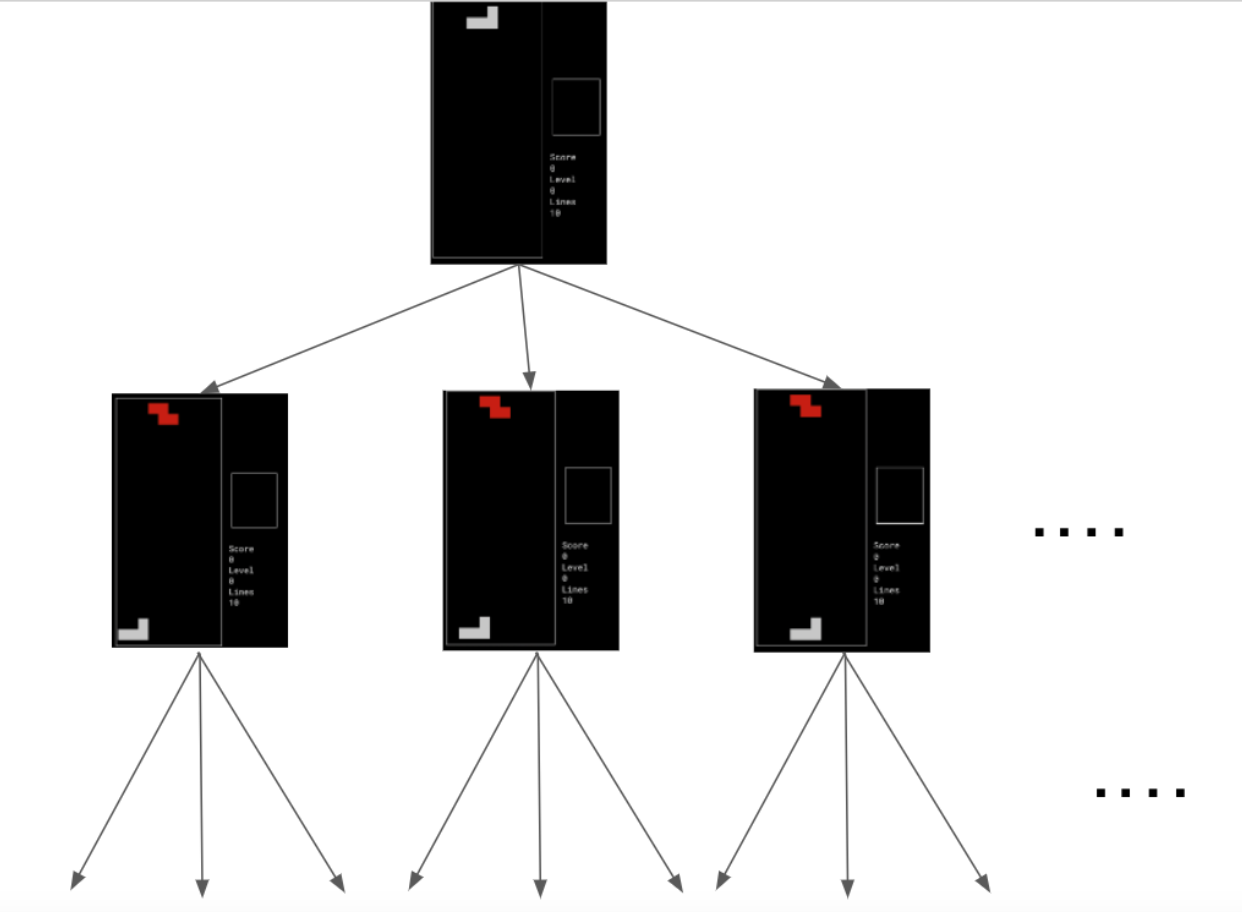
\includegraphics[width=0.3\textwidth]{search_space.png}
	\vspace{-1em}
	\caption{Tetris game search tree.}
	\label{fig:search_space}
\end{figure}

To evaluate a state for the search algorithm, we defined some evaluation metrics related to the tetris game such as the maximum height of the stacked blocks, holes in the game board not filled by blocks and lines cleared. The evaluation score is a weighted sum of these metrics, and is used to help the algorithm select the optimal position and orientation of the next move. We conducted experiments to obtain a set of weights that performed the best on achieving the highest score, which is used in guiding our search algorithms. Since this is not related to the parallelization of the search algorithms, we omit the details in our report.

\begin{figure}[h]
	\centering
	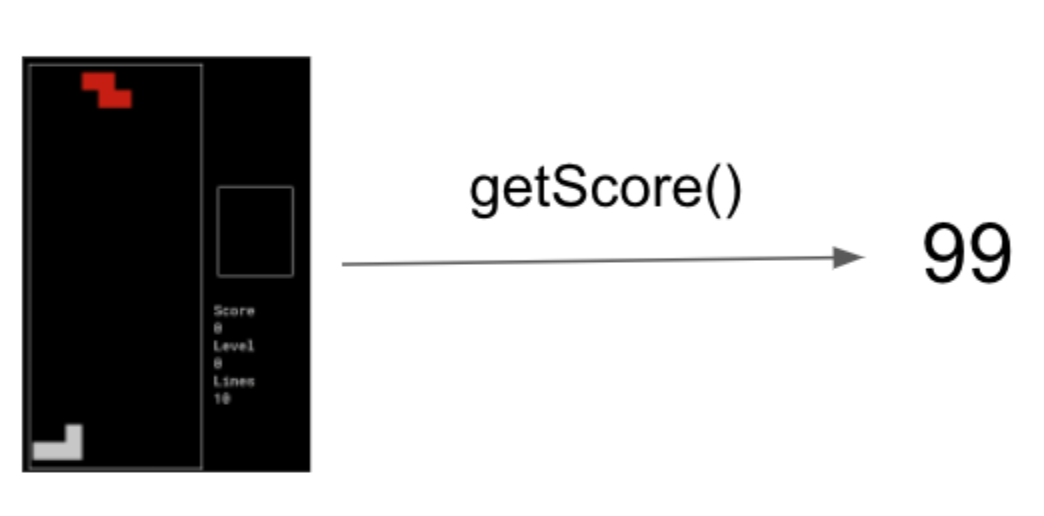
\includegraphics[width=0.2\textwidth]{score.png}
	\vspace{-1em}
	\caption{Score of tetris game state.}
	\label{fig:score}
\end{figure}

Our implementation is based on a tetris game repository (\ref{ref:tetrisRepo}) implemented in C on Github. We adopted its code for the game-play and game settings. Given the next four blocks to be dropped, we implemented solvers that calculate the next best orientation and position to place a tetris block, and supply it to the game. 

\begin{comment}

\subsection{Selecting a Template (Heading 2)}

First, confirm that you have the correct template for your paper size. This template has been tailored for output on the US-letter paper size. Please do not use it for A4 paper since the margin requirements for A4 papers may be different from Letter paper size.

\subsection{Maintaining the Integrity of the Specifications}

The template is used to format your paper and style the text. All margins, column widths, line spaces, and text fonts are prescribed; please do not alter them. You may note peculiarities. For example, the head margin in this template measures proportionately more than is customary. This measurement and others are deliberate, using specifications that anticipate your paper as one part of the entire proceedings, and not as an independent document. Please do not revise any of the current designations.

\end{comment}
\vspace{0.5em}
\section{Approach}

% APPROACH: Tell us how your implementation works. Your description should be sufficiently detailed to provide the course staff a basic understanding of your approach. Again, it might be very useful to include a figure here illustrating components of the system and/or their mapping to parallel hardware.
% Describe the technologies used. What language/APIs? What machines did you target?
% Describe how you mapped the problem to your target parallel machine(s). IMPORTANT: How do the data structures and operations you described in part 2 map to machine concepts like cores and threads. (or warps, thread blocks, gangs, etc.)
% Did you change the original serial algorithm to enable better mapping to a parallel machine?
% If your project involved many iterations of optimization, please describe this process as well. What did you try that did not work? How did you arrive at your solution? The notes you’ve been writing throughout your project should be helpful here. Convince us you worked hard to arrive at a good solution.
% If you started with an existing piece of code, please mention it (and where it came from) here.

In this section, we describe the implementation and parallelization of the tetris game solvers. First, we implemented sequential versions of depth-first search and breadth-first search solvers from scratch in C to be incorporated into the tetris game code \ref{ref:tetrisRepo}. Then, we parallelized both methods with OpenMP on the GHC machines and later conducted our experiments on the PSC bridges2 machines. We also built CilkPlus (\ref{ref:CilkPlus}) on the GHC machines and parallelized our DFS search algorithm with CilkPlus to alleviate workload imbalance.

The sequential version of our DFS and BFS solvers take the current game state as the input, which includes the game board as a char array and the next four tetris blocks to be dropped, and calculate 4 steps ahead for the best orientation and position to place the next tetris block. The best orientation and position is returned to the game code, where necessary game functions are executed to place the falling block to the best position and advance the game.

Specifically, we make a copy of the current tetris game object, which includes the current and next four falling blocks and the current game board as a 22x10 char array. The copy is passed to the solvers. Then, we perform game functions such as moving and dropping blocks on the tetris game object copy, which updates the game board. We calculate the resulting scores and other performance metrics and return the best orientation and position for the block back to the game.

For BFS, we need to store all states on a level of the search space in a queue, to be applied to the game board when we go deeper into the next level of the search space. This takes up a lot of memory space when there are four levels of the search tree, which makes it difficult to scale. In comparison, DFS is much better suited for this task in that it does not have to remember all states on a level. We now describe the parallelization approaches we took to parallelize both search algorithms.

\subsection{Approach 1}

Our first approach involves parallelizing both our DFS and BFS solvers with OpenMP on the GHC and PSC machines.

For the BFS approach, we created separate queues for the different threads and distributed the first layer nodes to different queues to run BFS. However, this approach suffers from memory problems because we need to store all possible states for BFS, as mentioned above.

For the DFS version, we parallelized the first layer nodes of the DFS search space. Initially, this produced sub-linear speedup with regard to the number of threads. However, we found out that the bottleneck was the C random function, because it requires mutual exclusion according to the source code, as shown in Fig \ref{fig:random_function}.

\begin{figure}[h]
	\centering
	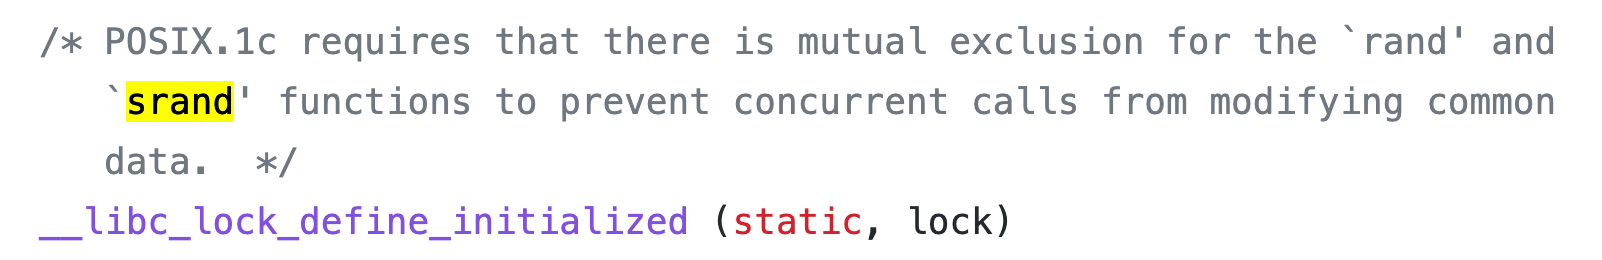
\includegraphics[width=0.4\textwidth]{random_function.png}
	\vspace{-1em}
	\caption{Random function bottleneck}
	\label{fig:random_function}
\end{figure}

As a result, we removed it when running the solver. This produced linear speedup up to 40 threads (on the psc machine), which is the number of first layer nodes. The graphs for search time and speedup with the increase of threads is shown in Fig \ref{fig:search_time_1} and Fig \ref{fig:speedup_1}, respectively. A problem with this approach is that it is difficult to parallelize with more threads using the current method because the number of first layer nodes is limited to 40. This is a major shortcoming since we should be able to perform 128-thread parallelization and much better speedup on the psc machines. To solve this issue, we decided on two alternative ways to perform parallelization: 1) rewrite the DFS parallel solver to map the workload onto the available threads (128 on the psc machines) and 2) perform the parallelization with Cilk instead of OpenMP. This brings us to our next approaches.

\subsection{Approach 2}

In this approach, instead of using DFS, we first calculate the number of possible leaf nodes, in the most naive case, it would be $40^{4}$ nodes. We then index this $40^{4}$ nodes and assign partition of the index to the worker threads where each worker thread is responsible for their assigned partition. For example, if there are 2560000 ($40^{4}$) nodes, each thread would be assigned 20000 nodes, so threads 0 would be responsible for node 0-19999, thread 1 responsible for node 20000-39999, and so on. Now the next problem is how do we map the node to the orientation and column position that should be dropped? We solve this by coming up with a one by one mapping function from the orientations and drop column position to the node id. We first consider there are four next blocks $T_{1}$, $T_{2}$, $T_{3}$ and $T_{4}$. Since we might prune redundant position, a tetris block might have less than 40 possible position. We let $O_{i}$ and $C_{i}$ be the number of possible orientation and drop column of tetromino block $T_{i}$, then the number of possible position of $T_{i}$ would be $O_{i} \cdot C_{i}$ which we annotate as $P_{i}$. Now the number of possible placement of all fours blocks would be $P_{1} \cdot P_{2} \cdot P_{3} \cdot P_{4}$. The next thing we do is we map the orientation $o_{i}$ and drop column $c_{i}$ of $T_{i}$ to a integer $tid_{i}$ where we define it as the tetris block id. We can achieve this easily by defining $$tid_{i} = o_{i} \cdot C_{i} + c_{i}$$ where both $o_{i}$, $c_{i}$ are integer and $o_{i} \in \interval[{0,O_{i}-1]$, $c_{i} \in \interval[{0,C_{i}-1]$.
Now consider the DFS case, every leaf node actually represent a combination of $tid_{i}$, hence we can map a leaf node to a set $\{ tid_{1}, tid_{2}, tid_{3},tid_{4}\}$. Finally, we can map this set to the node id we defined previously by the formula $$ id_{node} = tid_{1} \cdot  P_{2} \cdot P_{3} \cdot P_{4} + tid_{2} \cdot P_{3} \cdot P_{4} + tid_{3} \cdot P_{4} + tid_{4}$$
Using the formula, workers threads can easily map their given node id to the corresponding tetromino block placements using division and modulus. The synchronization overhead in this approach is neglectable since all threads first store the optimal solution of their partition to a local variable. The local optimal solution is then compared in a critical section to get the global optimal, which is very fast since it needs only the number of threads amount of comparison. This approach is much more flexible than approach one since we are now partitioning the node ids which is trivial to do, and allows us to do various optimization on the search space without changing our algorithm. It is also more efficient implementation-wise since we only need to recover the board state every 4 steps, unlike in the DFS case, where we need to do this for every new node. In the final version, we applied various optimization to push the perforamce to the limit, we would discuss them in the following section.
\subsection{Approach 3}

The other alternative for increasing the number of parallelization threads is to use Cilk. Cilk is the ideal parallelization tool given the recursive nature of our DFS solver. One advantage is the simplicity to convert C code to utilize Cilk, and the second advantage has to do with the workload imbalance due to pruning the redundant states mentioned in the background section.

First, we built CilkPlus on the GHC machine by building our own llvm with cmake via miniconda. The modifications we made to convert the code to Cilk includes using $cilk\_for$ to parallelize across different states of a level of search space (different positions and orientations). For each level, the DFS algorithm has to compare the scores obtained across different threads to find the optimal position and orientation. At first, we collected the scores from all threads using an array, and synchronized the threads with the $cilk\_sync$ barrier before performing a serialized comparison for all scores to find the best one. Then, we found that the cilk reducer \ref{ref:CilkReducer}, which is available only in C++, could be used to perform the same function without using synchronization and serialized comparison. Switching to the Cilk reducer speeds up the search time and reduces the amount of memory used since we do not need to keep track of scores form all threads.

Since there are redundant states as mentioned above, pruning them for optimization would cause workload imbalance. This would not be a problem with Cilk, since it has a work-stealing scheduler that would automatically balance the workload. A small problem we encountered is that we could not manually install CilkPlus on the PSC machines as we did on the GHC machines, because the gcc versions on the PSC machines are too recent. Therefore, we did not conduct our experiments of this approach on the PSC machines.


\section{Challenges \& Optimization}
\vspace{-0.5em}
In this section, we bring up some challenges and performance bottleneck we encounter that limited our speedup and how we optimized these bottlenecks. There are in total three optimization we performed.

\subsection{Redundant search space}
The first bottleneck that limits our speedup and performance is that there were a lot of redundant search state we are searching over. Our naive approach iterated over 4 orientation of each block, however, some tetromino blocks has less than 4 orientations. For example consider the I space tetromino block in Fig. \ref{fig:piece_orientation}.
\begin{figure}[h]
	\centering
	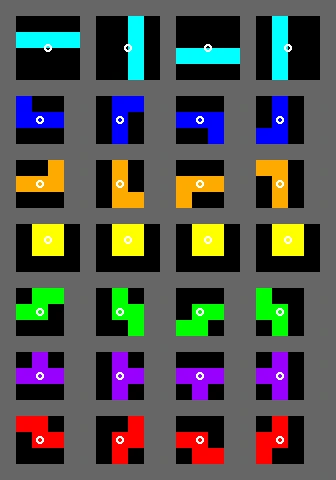
\includegraphics[width=0.2\textwidth]{SRS-pieces.png}
	\vspace{0em}
	\caption{Orientation of Tetromino Blocks. This figure shows orientation 0 to orientation 3 of all blocks from left to right}
	\label{fig:piece_orientation}
\end{figure}
It only has two unique orientations 0 and 1, the rest are just duplicate orientations. Secondly, we also assume that each block has 10 possible columm placement, which is obvious also not true since the shape of the block would limit its placement. For example, a I space block with orientation 0, would only have 6 possible column placement, otherwise the piece would go out of bound (under our game setting with column width as 10). Therefore, we were able to prune a lot of search space out, and each tetromino block has their own branching factor shown in Fig \ref{fig:tetris_table}.
\begin{figure}[h]
	\centering
	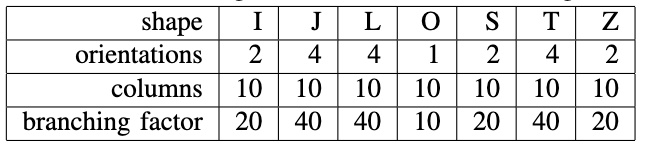
\includegraphics[width=0.5\textwidth]{tetris_table.png}
	\vspace{-1em}
	\caption{Branching Factor of Tetromino Blocks. Image reference: \ref{ref:tetrisImage}}
	\label{fig:tetris_table}
\end{figure}

% reference https://tetris.fandom.com/wiki/SRS?file=SRS-pieces.png
This optimization, however, can only be used in approach 2, otherwise it would introduce severe workload imbalance in the DFS tree, resulting in significant decrease in the speedup. In approach 2, since we are partitioning the combination space, it is easy for us to implement this but only on the orientations. We still iterate over 10 column for every blocks for coding simplicity. 

\subsection{Workload imbalance}
Here we focus on the workload imbalance of Approach 2. As mentioned previously, approach 2 can evenly partition the search space among worker threads. However, we still observed workload imbalance in the scoring phase of each worker where we take the tetris board state and output a score that indicates the wellness of the board. The imbalance is subtle but became a bottleneck when we optimized our code to a certain extent. We discovered that it was due to the function that calculates the height of each board. Since the way we find the height is checking from top to bottom of whether each row is empty and return if we found one non-empty row, this would result in a imbalance when the height of the board is different. Considering how we partitioned our search space, each threads would be responsible for a continuous range of node id thus the final board state of a thread would be similar. If one threads tends to always have a higher board state than another thread, its workload on the scoring phase would be higher resulting in a imbalance (see Fig \ref{fig:tetris_board}.) 
We solve this issue by simply storing the board height in the game object and maintaining it every time we place a tetromino on the board. This way we can get the height in constant time for any board state.
\begin{figure}[h]
	\centering
	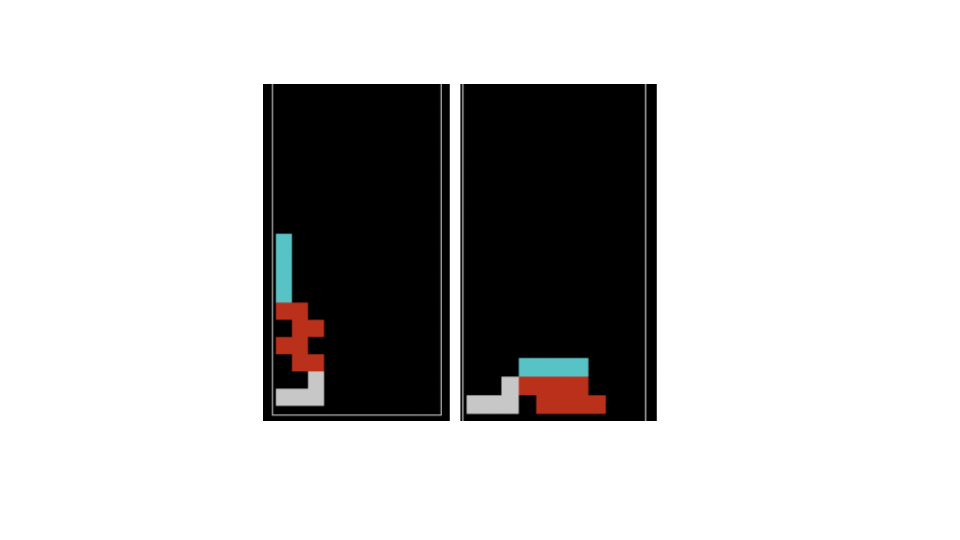
\includegraphics[width=0.5\textwidth]{tetris_board.png}
	\vspace{-3em}
	\caption{Low and High Tetris Board of Same Block Combination}
	\label{fig:tetris_board}
\end{figure}

\subsection{State caching}
Another optimization we did is that we cached the board state to avoid duplicate drops. Consider one worker thread reponsible for node 0 to node 20000. Using the formula we derived earlier we can see that consecutive nodes would have the same prefix for their tid set. For example, if node 0 corresponds to $\{ tid_{1}, tid_{2}, tid_{3},tid_{4}\}$ then node 1 would correspond to $\{ tid_{1}, tid_{2}, tid_{3},tid_{4} + 1\}$. In this case, we could cache the drop result of $\{ tid_{1}, tid_{2}, tid_{3}\}$, and reuse it. In the best case, we can save up to 40 x 3 drops, where 40 is the branching factor of the fourth block and 3 corresponds to the previous 3 drops. Currently, we are only caching depth - 1 layer of drops, more aggressive caching is possible but are harder to implement, the current implementation already can significantly lower our drop time.

\section{Results}

% RESULTS: How successful were you at achieving your goals? We expect results sections to differ from project to project, but we expect your evaluation to be very thorough (your project evaluation is a great way to demonstrate you understood topics from this course). Here are a few ideas:
% If your project was optimizing an algorithm, please define how you measured performance. Is it wall-clock time? Speedup? An application specific rate? (e.g., moves per second, images/sec)
% Please also describe your experimental setup. What were the size of the inputs? How were requests generated?
% Provide graphs of speedup or execute time. Please precisely define the configurations being compared. Is your baseline single-threaded CPU code? It is an optimized parallel implementation for a single CPU?
% Recall the importance of problem size. Is it important to report results for different problem sizes for your project? Do different workloads exhibit different execution behavior?
% IMPORTANT: What limited your speedup? Is it a lack of parallelism? (dependencies) Communication or synchronization overhead? Data transfer (memory-bound or bus transfer bound). Poor SIMD utilization due to divergence? As you try and answer these questions, we strongly prefer that you provide data and measurements to support your conclusions. If you are merely speculating, please state this explicitly. Performing a solid analysis of your implementation is a good way to pick up credit even if your optimization efforts did not yield the performance you were hoping for.
% Deeper analysis: Can you break execution time of your algorithm into a number of distinct components. What percentage of time is spent in each region? Where is there room to improve?
% Was your choice of machine target sound? (If you chose a GPU, would a CPU have been a better choice? Or vice versa.)

\begin{figure}[h]
	\centering
	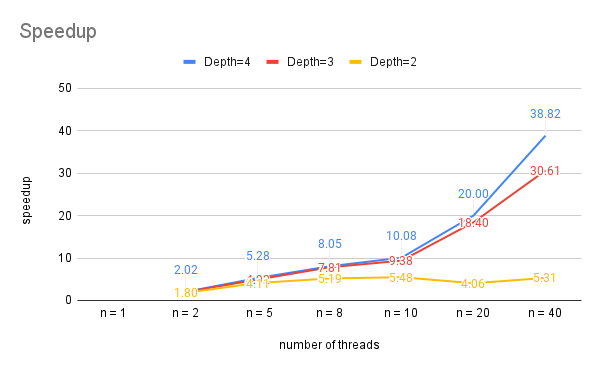
\includegraphics[width=0.45\textwidth]{speedup.png}
	\vspace{-1em}
	\caption{Approach 1 Speedup vs. Number of threads for different search depths. This figure shows that the speedup increases linearly with the number of threads.}
	\label{fig:speedup}
\end{figure}

\begin{figure}[h]
	\centering
	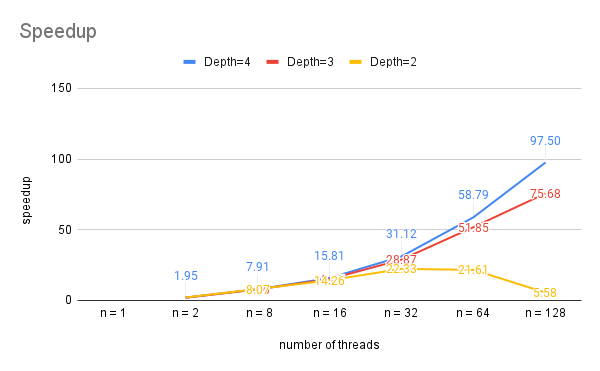
\includegraphics[width=0.45\textwidth]{Speedup_naive.png}
	\vspace{-1em}
	\caption{Approach 2 Naive Speedup vs. Number of threads for different search depths.}
	\label{fig:speedup_naive}
\end{figure}

\begin{figure}[h]
	\centering
	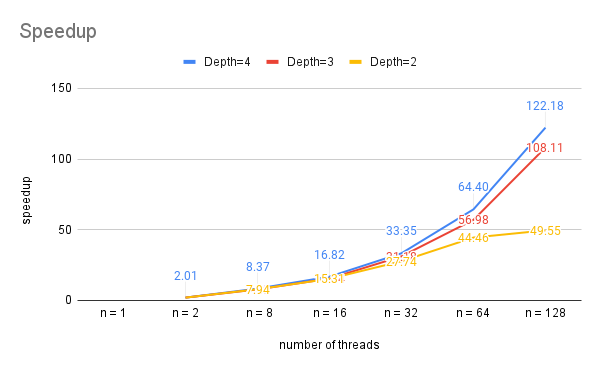
\includegraphics[width=0.45\textwidth]{Speedup_optimized.png}
	\vspace{-1em}
	\caption{Approach 2 Optimized Speedup vs. Number of threads for different search depths.}
	\label{fig:speedup_optimized}
\end{figure}

\begin{table}
\begin{tabular}{|l|r|r|r|r|r|}
\hline Depth 4 & \multicolumn{2}{|l|}{$\mathrm{n}=1$} & \multicolumn{2}{|l|}{$\mathrm{n}=128$} & ratio \\
\cline { 2 - 5 } & \multicolumn{1}{|l|}{ time(ms) } & pct(\%) & time(ms) & pct.(\%) & \\
\hline solve & $9534.483$ & $74.01 \%$ & $77.678$ & $71.29 \%$ & $1.25$ \\
\hline drop & $2451.974$ & $19.03 \%$ & $22.209$ & $20.38 \%$ & $1.61$ \\
\hline copy & $70.101$ & $0.54 \%$ & $0.591$ & $0.59 \%$ & $1.24$ \\
\hline create & 0 & $0.00 \%$ & $0.388$ & $0.36 \%$ & $5687.5$ \\
\hline other & $826.24$ & $6.41 \%$ & $8.1$ & $7.42 \%$ & $-$ \\
\hline total & $12882.80$ & $100.00 \%$ & $108.953$ & $100.00 \%$ & $1.27$ \\
\hline Depth 3 & \multicolumn{2}{|l|}{$\mathrm{n}=1$} & \multicolumn{2}{|l|}{$\mathrm{n}=128$} & ratio \\
\cline { 2 - 5 } & \multicolumn{1}{|l|}{ time(ms) } & pct(\%) & time(ms) & pct.(\%) & \\
\hline solve & $232.794$ & $77.54 \%$ & $1.892$ & $63.51 \%$ & $1.2$ \\
\hline drop & $45.863$ & $15.28 \%$ & $0.469$ & $15.74 \%$ & 2 \\
\hline copy & $1.752$ & $0.58 \%$ & $0.013$ & $0.59 \%$ & $6.36$ \\
\hline create & 0 & $0.00 \%$ & $0.396$ & $13.29 \%$ & $1045.8$ \\
\hline other & $19.81$ & $6.60 \%$ & $0.2$ & $7.02 \%$ & $-$ \\
\hline total & $300.22$ & $100.00 \%$ & $2.979$ & $100.00 \%$ & $1.68$ \\
\hline Depth 2& \multicolumn{2}{|l|}{$\mathrm{n}=1$} & \multicolumn{2}{|l|}{$\mathrm{n}=128$} & ratio \\
\cline { 2 - 5 } & \multicolumn{1}{|l|}{ time(ms) } & pct(\%) & time(ms) & pct.(\%) & \\
\hline solve & $5.803$ & $81.72 \%$ & $0.051$ & $13.32 \%$ & $94.5$ \\
\hline drop & $0.783$ & $11.03 \%$ & $0.007$ & $1.83 \%$ & $17.8$ \\
\hline copy & $0.043$ & $0.61 \%$ & $0.00034$ & $0.59 \%$ & $2.86$ \\
\hline create & 0 & $0.00 \%$ & $0.316$ & $82.51 \%$ & $395.4$ \\
\hline other & $0.47$ & $6.65 \%$ & $0.0$ & $2.26 \%$ & $-$ \\
\hline total & $7.10$ & $100.00 \%$ & $0.383$ & $100.00 \%$ & $116.5$ \\
\hline
\end{tabular}
\caption{function duration breakdown of naive approach 2.}
\label{tab:function_duration_naive}
\end{table}

\begin{table}
\begin{tabular}{|l|r|r|r|r|r|}
\hline Depth 4 & \multicolumn{2}{|l|}{$\mathrm{n}=1$} & \multicolumn{2}{|l|}{$\mathrm{n}=128$} & ratio \\
\cline { 2 - 5 } & \multicolumn{1}{|l|}{ time(ms) } & pct(\%) & time(ms) & pct.(\%) & \\
\hline solve & $8002.533$ & $79.05 \%$ & $62.937$ & $74.85 \%$ & $1.1$ \\
\hline drop & $1218.769$ & $12.04 \%$ & $12.376$ & $14.72 \%$ & $1.25$ \\
\hline copy & $70.227$ & $0.69 \%$ & $0.592$ & $0.70 \%$ & $1.48$ \\
\hline create & $0.001$ & $0.00 \%$ & $0.0002$ & $0.00 \%$ & $1.47$ \\
\hline other & $832.39$ & $8.22 \%$ & $8.2$ & $9.73 \%$ & $-$ \\
\hline total & $10123.93$ & $100.00 \%$ & $84.083$ & $100.00 \%$ & $1.09$ \\
\hline Depth 3 & \multicolumn{2}{|l|}{$\mathrm{n}=1$} & \multicolumn{2}{|l|}{$\mathrm{n}=128$} & ratio \\
\cline { 2 - 5 } & \multicolumn{1}{|l|}{ time(ms) } & pct(\%) & time(ms) & pct.(\%) & \\
\hline solve & $183.701$ & $77.63 \%$ & $1.543$ & $71.20 \%$ & $1.09$ \\
\hline drop & $31.128$ & $13.15 \%$ & $0.338$ & $15.60 \%$ & $1.4$ \\
\hline copy & $1.766$ & $0.75 \%$ & $0.014$ & $0.65 \%$ & $5.14$ \\
\hline create & $0.0001$ & $0.00 \%$ & $0.00009$ & $0.00 \%$ & $1.154$ \\
\hline other & $20.03$ & $8.47 \%$ & $0.3$ & $12.55 \%$ & $-$ \\
\hline total & $236.63$ & $100.00 \%$ & $2.167$ & $100.00 \%$ & $1.11$\\
\hline Depth 2& \multicolumn{2}{|l|}{$\mathrm{n}=1$} & \multicolumn{2}{|l|}{$\mathrm{n}=128$} & ratio \\
\cline { 2 - 5 } & \multicolumn{1}{|l|}{ time(ms) } & pct(\%) & time(ms) & pct.(\%) & \\
\hline solve & $4.578$ & $77.88 \%$ & $0.039$ & $32.50 \%$ & $75.96$ \\
\hline drop & $0.778$ & $13.24 \%$ & $0.009$ & $7.50 \%$ & $38.58$ \\
\hline copy & $0.043$ & $0.73 \%$ & $0.0003$ & $0.25 \%$ & $2.86$ \\
\hline create & $0.00006$ & $0.00 \%$ & $0.0001$ & $0.08 \%$ & $1.09$ \\
\hline other & $0.48$ & $8.15 \%$ & $0.1$ & $59.67 \%$ & $-$ \\
\hline total & $5.88$ & $100.00 \%$ & $0.12$ & $100.00 \%$ & $1.12$\\
\hline
\end{tabular}
\caption{function duration breakdown of optimized approach 2.}
\label{tab:function_duration_optimized}
\end{table}
In this section, we present the results for the experiments we conducted on the GHC and PSC machines. We focused our experiments on approach2 since it has the best performance and also the most flexible design. 

\subsection{Approach 1 Naive DFS}
Our first experiment measures the speedup with different number of threads for the approach 1 parallelized OpenMP DFS search algorithm for different search depths. A graph of the experiment is shown in Fig. \ref{fig:speedup}. Here we only show the speedup up to 40 threads since the DFS algorithm can't support threads more than 40. We can observe from the graph that as the search depth increases, the speedup approaches linear speedup to the number of threads used. We think the reason is that shallower depth results in smaller search space and the overhead of searching for the optimal position and orientation outweighs the speedup benefits. However, later we discover that the main reason for the sub-optimal speedup is because of a lock shared between the threads which we would discuss in later sections. Since this approach limited the number of thread we can use, we didn't further optimize this approach.

\subsection{Approach 2 Before Optmization}
The next experiment measures the speedup with different number of threads for the Approach 2 parallelized method for different search depths. The graph of this experiment is shown in Fig. \ref{fig:speedup_naive}. This experiment is conducted on n=1 to n=128 threads. We can observe the same trend of speedup approaching linear to the number of threads used as the search depth increases. However, the speedup is not perfect for n = 64 and n = 128. This is due to the workload imbalance we mentioned in the previous section. As for depth = 2, we observed the same performance downgrade in the Approach 1 for high number of threads. 

To further investigate the non-linear speedup for shallower search depths, we conduct our third experiment, which measures the duration of each function. The results of this experiment is displayed in Table. \ref{tab:function_duration_naive}. For this experiment, we measure the execution time of four main functions that is necessary during our DFS search for different search depths using 1 and 128 threads, respectively. We used C function gettimeofday which has the granularity of microseconds. The overhead of the time measurement is under 1us so wouldn't affect the solver performance. 
In the table, we measure 4 crucial function including solve, drop, copy and create. The solve function denotes the tg\_get\_score() function, which is used to calculate the score of a game state. The drop function denotes the tg\_drop() function, which drops the falling block into place after the block position (column) has been determined. The copy function denotes the tg\_copy() function, which copies the tetris game solver, this is needed because we want to resume the board state. The create function denotes the tg\_create() function, which creates a new tetris game solver function. We measured tg\_create() because we discovered it was the bottleneck for shallower depth, especially for depth = 2. 
Additionally, we also measure the maximum and minimum execution time of each function between different threads and define ratio as maximum / minimum, the larger ratio is, the more imbalance the function workload is.  

We can observe from Table. \ref{tab:function_duration_naive} for depth 3 and 4, most execution time is on solve and drop accounting for over 85\% of the work time, which is what we expected. However, there is a slight workload imbalance of the two function (1.2 and 1.6 for depth = 4) that limits our speedup from reaching perfect speedup. The overhead of multiple threads here are still small with around 7\% of total time. As for depth = 2, we can see that the execution time is mostly on tg\_create() which is abnormal. The ratio of tg\_create() in all depth is also unreasonably large. After some dig in, we find that it was because the same problem we encounter earlier, there was a srand() function call in tg\_create() that acquires a lock betweens threads. Therefore, we removed this srand() in the optimized version of approach 2. 

\subsection{Approach 2 After Optimization}
Here we present the result of our optimized approach 2, we applied the three optimization mentioned in optimization section and also fixed the srand() locking problem. The speedup result is shown in Fig. \ref{fig:speedup_optimized}. We can see that depth = 4 reached near perfect speedup (122.18) after we optimized the workload imbalance of the tg\_get\_score() function. As the depth decrease, the overheads takes in effect and the speedup is lowered, as depth = 2 has only 49.55 speedup, however this is still much higher than the naive version (5.41). 

From Table. \ref{tab:function_duration_optimized} there is 4 things worth pointing out. First, the tg\_create() is no longer a bottleneck for depth = 2 n = 128, instead other are now the main reason for the performance slowdown. This is expected since we fixed the lock problem. Second, as the depth decrease, the other percentage also increase, especially in depth = 2, where 60\% of the time is on other. This is expected since other represents the overhead and the overhead increase as depth decrease since we have less calculation for each thread. Third, the drop function time for depth = 4 decreased from 20\% to 15\%, indicating our caching is effective. Finally, we can see that nearly all ratio decrease for all depth, which implies that our optimization has successfully solve the workload imbalance, resulting in better speedup. 

\addtolength{\textheight}{-12cm}
% Balance the column lengths on the last page
\section{Conclusion}
In this project, we present and analyzed several way to implement a tetris solver, including a approach (approach 2) that partitions the tetris search space evenly making it extremely easy to parallelize our solver. We then analyzed the performance bottleneck and reasons for imperfect speedup and proposed 3 optimizations. After applying our optimizations, we show that we removed nearly all workload imbalance and increased our speedup to near perfect speedup. To prove our result, we measured and analyzed the time spent on each critical functions using gettimeofday(). 
As a result, we were able to build a tetris solver that can clear up to 1000 lines per second.
\vspace{0.5em}
\begin{thebibliography}{99}

\bibitem{c1}\label{ref:tetrisGame} https://en.wikipedia.org/wiki/Tetris

\bibitem{c2}\label{ref:tetrisRepo} https://github.com/brenns10/tetris

\bibitem{c3}\label{ref:CilkPlus} https://cilkplus.github.io

\bibitem{c4}\label{ref:tetrisImage} https://tetris.fandom.com/wiki/SRS?file=SRS-pieces.png

\bibitem{c5}\label{ref:Genetic} Man, Kim-Fung, Kit-Sang Tang, and Sam Kwong. "Genetic algorithms: concepts and applications [in engineering design]." IEEE transactions on Industrial Electronics 43.5 (1996): 519-534.

\bibitem{c6}\label{ref:Minimax} Korf, Richard E., and David Maxwell Chickering. "Best-first minimax search." Artificial intelligence 84.1-2 (1996): 299-337.

\bibitem{c7}\label{ref:CilkReducer} Frigo, Matteo, et al. "Reducers and other Cilk++ hyperobjects." Proceedings of the twenty-first annual symposium on Parallelism in algorithms and architectures. 2009.

\bibitem{c8}\label{ref:TetrisHard} Demaine, Erik D., Susan Hohenberger, and David Liben-Nowell. "Tetris is hard, even to approximate." International Computing and Combinatorics Conference. Springer, Berlin, Heidelberg, 2003.

\bibitem{c9}\label{ref:MonteCarlo} Galván-López, Edgar, et al. "Heuristic-based multi-agent monte carlo tree search." IISA 2014, The 5th International Conference on Information, Intelligence, Systems and Applications. IEEE, 2014.

\bibitem{c10}\label{ref:AlphaBeta} Singhal, Shubhendra Pal, and M. Sridevi. "Comparative study of performance of parallel Alpha Beta Pruning for different architectures." 2019 IEEE 9th International Conference on Advanced Computing (IACC). IEEE, 2019.

\bibitem{c11}\label{ref:Burgiel} Burgiel, Heidi. "How to lose at Tetris." The Mathematical Gazette 81.491 (1997): 194-200.

\begin{comment}

\bibitem{c1} G. O. Young, ÒSynthetic structure of industrial plastics (Book style with paper title and editor),Ó 	in Plastics, 2nd ed. vol. 3, J. Peters, Ed.  New York: McGraw-Hill, 1964, pp. 15Ð64.
\bibitem{c2} W.-K. Chen, Linear Networks and Systems (Book style).	Belmont, CA: Wadsworth, 1993, pp. 123Ð135.
\bibitem{c3} H. Poor, An Introduction to Signal Detection and Estimation.   New York: Springer-Verlag, 1985, ch. 4.
\bibitem{c4} B. Smith, ÒAn approach to graphs of linear forms (Unpublished work style),Ó unpublished.
\bibitem{c5} E. H. Miller, ÒA note on reflector arrays (Periodical styleÑAccepted for publication),Ó IEEE Trans. Antennas Propagat., to be publised.
\bibitem{c6} J. Wang, ÒFundamentals of erbium-doped fiber amplifiers arrays (Periodical styleÑSubmitted for publication),Ó IEEE J. Quantum Electron., submitted for publication.
\bibitem{c7} C. J. Kaufman, Rocky Mountain Research Lab., Boulder, CO, private communication, May 1995.
\bibitem{c8} Y. Yorozu, M. Hirano, K. Oka, and Y. Tagawa, ÒElectron spectroscopy studies on magneto-optical media and plastic substrate interfaces(Translation Journals style),Ó IEEE Transl. J. Magn.Jpn., vol. 2, Aug. 1987, pp. 740Ð741 [Dig. 9th Annu. Conf. Magnetics Japan, 1982, p. 301].
\bibitem{c9} M. Young, The Techincal Writers Handbook.  Mill Valley, CA: University Science, 1989.
\bibitem{c10} J. U. Duncombe, ÒInfrared navigationÑPart I: An assessment of feasibility (Periodical style),Ó IEEE Trans. Electron Devices, vol. ED-11, pp. 34Ð39, Jan. 1959.
\bibitem{c11} S. Chen, B. Mulgrew, and P. M. Grant, ÒA clustering technique for digital communications channel equalization using radial basis function networks,Ó IEEE Trans. Neural Networks, vol. 4, pp. 570Ð578, July 1993.
\bibitem{c12} R. W. Lucky, ÒAutomatic equalization for digital communication,Ó Bell Syst. Tech. J., vol. 44, no. 4, pp. 547Ð588, Apr. 1965.
\bibitem{c13} S. P. Bingulac, ÒOn the compatibility of adaptive controllers (Published Conference Proceedings style),Ó in Proc. 4th Annu. Allerton Conf. Circuits and Systems Theory, New York, 1994, pp. 8Ð16.
\bibitem{c14} G. R. Faulhaber, ÒDesign of service systems with priority reservation,Ó in Conf. Rec. 1995 IEEE Int. Conf. Communications, pp. 3Ð8.
\bibitem{c15} W. D. Doyle, ÒMagnetization reversal in films with biaxial anisotropy,Ó in 1987 Proc. INTERMAG Conf., pp. 2.2-1Ð2.2-6.
\bibitem{c16} G. W. Juette and L. E. Zeffanella, ÒRadio noise currents n short sections on bundle conductors (Presented Conference Paper style),Ó presented at the IEEE Summer power Meeting, Dallas, TX, June 22Ð27, 1990, Paper 90 SM 690-0 PWRS.
\bibitem{c17} J. G. Kreifeldt, ÒAn analysis of surface-detected EMG as an amplitude-modulated noise,Ó presented at the 1989 Int. Conf. Medicine and Biological Engineering, Chicago, IL.
\bibitem{c18} J. Williams, ÒNarrow-band analyzer (Thesis or Dissertation style),Ó Ph.D. dissertation, Dept. Elect. Eng., Harvard Univ., Cambridge, MA, 1993. 
\bibitem{c19} N. Kawasaki, ÒParametric study of thermal and chemical nonequilibrium nozzle flow,Ó M.S. thesis, Dept. Electron. Eng., Osaka Univ., Osaka, Japan, 1993.
\bibitem{c20} J. P. Wilkinson, ÒNonlinear resonant circuit devices (Patent style),Ó U.S. Patent 3 624 12, July 16, 1990. 
\end{comment}


\end{thebibliography}
\section{LIST OF WORK BY EACH STUDENT, AND DISTRIBUTION OF TOTAL CREDIT}
We implemented nearly every function together.

Yen Li Laih (ylaih): 50\%
Wei Wei Lin (weiweil2): 50\%

\end{document}